
%!TEX TS-program = xelatex
%!TEX encoding = UTF-8 Unicode

\documentclass[12pt]{article}
\usepackage{geometry}                
\geometry{letterpaper}                   
\usepackage{amsmath}
\usepackage{graphicx}
\usepackage{amssymb}
\usepackage{tikz}
\usepackage{framed}
\usepackage{listings}
\lstset{language=Octave,
  basicstyle=\footnotesize,
  tabsize=3,
  language=python,
  breaklines=true,
  mathescape=true,
  commentstyle=\color{blue},
  morecomment=[l]{\#}}



\author{Elliott Hauser}
\title{Comp 555 Problem Set 4}
\begin{document}
\maketitle

\section*{Question 1}
1. Consider the following four sequences 
Chimp GTTG
Gorilla  GTCA
Human  ACCA
Orangutan ATTA
Assume the following scoring matrix
  A T G C
A 0 2 3 8
T 2 0 1 3
G 3 1 0 3
C 8 3 3 0

\paragraph{a.} % (fold)
\label{par:1a}
Six binary tree topologies with two different tree structures are shown in Figure~\ref{trees}. 

\begin{figure}[htb]
	\begin{center}
		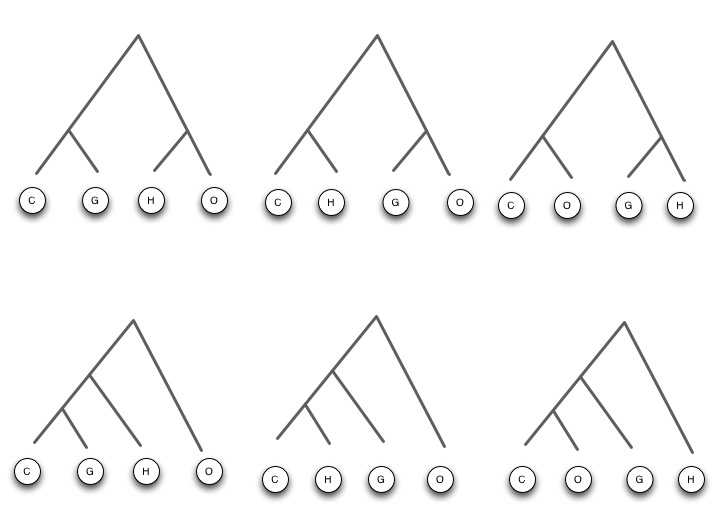
\includegraphics[width=5in]{trees.jpg}
	\end{center}
	\caption{Six binary tree topologies, utilizing two different tree structures.}
	\label{trees}
\end{figure}

\paragraph{b.} % (fold)
\label{par:1b}
b. Apply Sankoff’s algorithm to the topologies created in (a) to 
determine the weighted parsimony score. What is the minimum parsimony 
score? What is the most plausible topology of the six you created? 
Why?
% paragraph b_ (end)

\paragraph{c.} % (fold)
\label{par:1c}


c. Apply Fitch’s algorithm to the same topologies. Find the sequences 
for the roots for all. Which is the one with the least parsimony 
score. 
% paragraph paragraph_name (end)
d. Do b) and c) give same results. Why or Why not?


\section*{Question 2}
2. Consider the following distance matrix
  A  B  C  D  E  F
A 0 18 15 21  6 16
B    0 23 19 20 24
C       0 26 17 19
D          0 23 27
E             0 18
F                0



1,1,2,1,2,1
\paragraph{a.} % (fold)

% a) Is this distance matrix additive ? Why or why not?
A matrix is additive if there exists a tree $T$ with $d_{i,j}(T) = D_{i,j}$.  But an efficient way to determine this is the Four point theorem, which states that, for every combination of leaves $i$, $j$, $k$, and $l$, the sums $D_{i,j}, D_{j,k},$ and $ D_{k,l}$ yeild two identical sums, with the third sum smaller than these two.

To test this, I wrote a simple algorithm in Python.  It is shown in Figure~\ref{fourpoint}

\begin{figure}[htb]
	\centering
	\begin{lstlisting}[language=Python]
def four_point():

	mismatch = []

	for i in xrange(0,5):
		for j in xrange(0,5):
			if i == j:
				continue
			for k in xrange(0,5):
				if k == j:
					continue
				if k == i:
					continue
				for l in xrange(0,5):
					if l == k:
						continue
					if l == j:
						continue
					if l == i:
						continue
					one = matrix[i][j] + matrix[k][l]
					two = matrix[i][k] + matrix[j][l]
					three = matrix[i][l] + matrix[j][k]
					lump = [one,two,three]
					together = set(lump)
					if len(together) != 2:
						print i,j,k,l
						print lump
						print matrix[i][j]," + ",matrix[k][l]," = ",one
						print matrix[i][k]," + ",matrix[j][l]," = ",two
						print matrix[i][l]," + ",matrix[j][k]," = ",three
						print together
	\end{lstlisting}
	\caption{An algorithm to calculate whether the four point condition holds for an $n\times n$ matrix.}
	\label{fourpoint}
\end{figure}

% paragraph paragraph_name (end)


\paragraph{b.} % (fold)
\label{par:b_}
% b) Design an efficient method to determine “delta” for an iteration. 



% paragraph b_ (end)
\paragraph{c.} % (fold)
\label{par:paragraph_name}
% c) Find “delta” and i,j,k for the first two iterations.


% paragraph .c (end)
\clearpage
\section*{Question 3}
For this problem let us define $i$ as the number of islands connected in a graph of arbitrary vertices. In this problem, $i=8$. Figure~\ref{twographs} shows an initial formulation of the boundaries of the problem of visiting each island.  On the left, the minumum possible trips are shown, which are $i-1 =7$.  On the right is an arrangement where the maximum number of trips must be taken.  Because of the inclusion of a central hub, many routes must be taken more than once.  In fact, were we not able to choose our starting island in this problem, this example would disprove the desired limit of 12 since the trip length is $((i-2)*2)-1=13$. 
But the problem places no such restriction on us, and so the minumum number of trips in the pathological case is show in Figure~\ref{onegraph}, and is $((i-1)*2)-2=12$.  How can we prove that this is the maximum number of trips?  The graph shown on the right in Figure~\ref{twographs} and in Figure~\ref{onegraph} is pathological because there are the maximum amount of nodes connected by only one edge, 7, which is $i-1$, i.e. all nodes except the central node.  Each of these potentially requires two trips to visit and then keep visiting other islands, yielding $(i-1)*2=14$  But we know that all of the islands are visited before each vertex is traveled twice.  In fact, if one both starts and ends on one of the outlying islands as int he irght of Figure~\ref{onegraph}, two of these return trips can be eliminated, one each for the Start and End islands, giving us the answer of $((i-1)*2)-2=12$.  Starting on the central island, as in the right of Figure~\ref{twographs} eliminates only one of these return trips, yielding $((i-1)*2)-1=13$.

\begin{figure}[htb]
	\begin{center}
		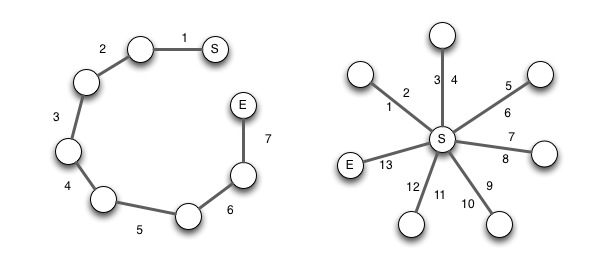
\includegraphics[width=4.5in]{twographs.jpg}
	\end{center}
	\caption{Initial formulation of the problem.  The tree on the left shows the minimum trips possible to visit all islands (i, while the tree on the right shows the pathological case where the maximum amount of trips must be taken if the starting islands cannot be chosen.  Start and end positions are marked by S and E, respectively, and trips are numbered.}
	\label{twographs}
\end{figure}


\begin{figure}[htb]
	\begin{center}
		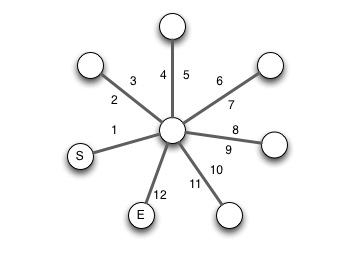
\includegraphics[width=3in]{onegraph.jpg}
	\end{center}
	\caption{The shortest path visiting all islands in the pathological case, where the starting islands are able to be chosen.  Its length is $(i-1)*2 - 2 = 12$}
	\label{onegraph}
\end{figure}

\clearpage

\section*{Question 4}
% Book 11.6
\paragraph{a}  The hidden markov model for this porblem is in Figure~\ref{hmm}

\begin{figure}[htb]
	\begin{center}
		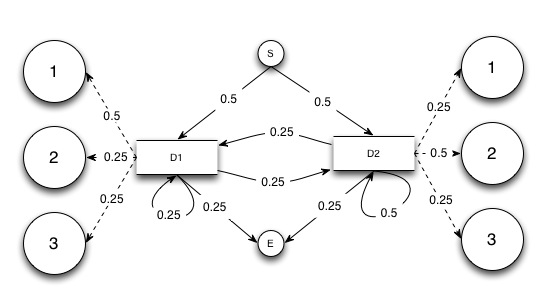
\includegraphics[width=4.5in]{hmm.jpg}
	\end{center}
	\caption{A hidden markov model of $Q=\textit{start},D1,D2,\textit{end}$ and $\Sigma = 1,2,3$}
	\label{hmm}
\end{figure}

\section*{Question 5}
% 5. In problem 4 (book 11.6), for the sequence 112122, what is the 
% probability that third 1 came from die D1

The probability that state $k$ caused emission $x$ at moment $i$ is given by
\[
	 P(\pi_i = k|x) = \frac{f_{k}(i) \cdot b_k(i)}{P(x|\pi)}
\]
Also,
\[
	f_{k}(i) = e_k(x_i)\cdot \sum_{l\in Q} f_{l,i-1}\cdot a_{l,k} 
\]
and
\[
	b_{k}(i) = e_k(x_i)\cdot \prod_{l\in Q} f_{l,i-1}\cdot a_{l,k}
\]
Finally,
\[
	P(x)=\sum_\pi P(x|\pi)
\]
I calculate these three terms, respectively, as
$$\begin{array}{ccc}
	f_k(x_4)= \\
	b_k(x_4)= \\
	P(x) = 
\end{array}$$
This yields  % ############# need real numbers here.
\[
	P(\pi_i = k|x) = \frac{1 \cdot 1}{1}
\]
\end{document}
